\section{Evaluation of the Project}
Testing and evaluation were vital parts of the project, to ensure that the system contained all the functionality it should have, adhered to all the constraints place upon it and that it was actually usable. Three stages of testing were therefore conducted. The first of these was functionality testing, in which the functional requirements of the system would be evaluated, and the system would be tested to see whether or not it implemented this functionality. The next stage was non-functional testing, in which the non-functional requirements would be evaluated, to ensure the system abided by them. The final stage was user feedback testing, in which a group of participants would actually be using the system. In this stage, three systems would be evaluated: MATLAB, FuzzyToolkitUoN, and this project; in order to determine which provided a better user experience.

\subsection{Functional Testing}
In this section, each of the functional requirements laid out in section \ref{sec:funcs} have been evaluated in turn, to ensure the system meets them. Knowledge of the inner workings of the system is not actually necessary to understand these tests, as they simply check whether functionality is present, and are not concerned as to how the system actually implements it (this is known as black box testing \cite{beizer1995black}). A complete listing of all the tests conducted, and their results, can be found in appendix \ref{app-ctl}.

\subsection{Non-Functional Testing}
In this section, each of the non-functional requirements laid out in section \ref{sec:non-funcs} have been enumerated, and the success to which they have been achieved has been detailed. The purpose of this is to evaluate how well the system has adhered to the constraints placed upon it.

\paragraph{Accessibility}\ \\
This was one of the biggest goals for the system, as it was one of it's main reasons for conception. The problem with most fuzzy logic software systems currently is that they are difficult to use, or difficult to access. That is why the project proposed in this report has accessibility improvements as one of it's main goals. To accomplish this, the system is entirely web based. The advantage of this, is that the user can access the system from any computer, running any operating system. This cross compatibility greatly improves the outreach of the software, as no users will be unable to access it. Further to this, the system front end is constructed entirely in HTML, CSS, and JavaScript. This means that the user does not require the download of any additional software, or applications, to use this system (which would not be case if Adobe Flash, or Java had been used). 

\paragraph{Usability and Operability}\ \\
This is a goal of the system that is difficult to quantitatively measure. In order to actually test this goal, a set of participants of varying skill levels were asked to complete a list of tasks, using this system, and compare this to doing the same tasks in similar systems. The detailed results of these tests can be found in section \ref{sec:uft}. After the user feedback testing, it was found that the majority of participants preferred this new system, over the other two that were tested (MATLAB's fuzzy toolbox, and FuzzyToolkitUoN). The major reasons for this were the ``waterfall'' style to task completion (each task was laid out in a logical manner, and followed on smoothly from the last), and the clean, uncluttered user interface. 

\paragraph{Maintainability}\ \\
To aid with the eventual goal of the system back end being interchangeable with any back end that can process fuzzy logic, the system needed to be coded so that is was easily maintainable, and easily expandable. In order to achieve this, the code has been written in a modular fashion, split across multiple files. Each file deals with exactly one action (file manipulation, rule creation, evaluation, etc.), and thus adding new functionality should be relatively easy. Each function has been listed with the purpose of it, the parameters it takes (and their types), and the value it returns, if any. This means identifying the purpose of functions is extremely simple, and any maintainer will easily be able to interpret how the system works. 

\paragraph{Quality}\ \\
To ensure that this system reflects well both on myself, and the University of Nottingham, it was made to be of the highest quality possible. The system has been built with a vast quantity of error handling methods, so that the system should not crash under operation, and should function exactly as the user expects. Helpful, and positive, error messages accompany any error handling methods, so the user can rectify any mistakes they make (without feeling punished for making them). 

\paragraph{Resource Requirements and Constraints}\ \\
As the system is aimed at any level of user, no assumptions as to the level of hardware they may possess can be made. This means that the system must be built to be as light weight as possible, as to not overwhelm the user's device. Fortunately, the technologies used to build the front end (CSS, HTML and JavaScript) are relatively light weight, and the front end has minimal processing requirements. The main processing that takes place is on the server side, when inference occurs.

\paragraph{Cross Platform Compatibility}\ \\
As mentioned previously, the system is built with entirely cross compatible languages, and only requires the user have an internet connection, and a web browser installed to be accessed and used. Aside from these, there are no compatibility issues the system presents, as it is entirely web based, and requires no additional resources to function. There is potential that the system would not work on extremely old operating systems, but all operating systems that are currently being supported by their developers should function correctly.

\paragraph{Security}\ \\
In a web based system, there is potential for many security issues to be present. However, in this system, that is not the case, as it does not store any user data, and the only information stored on the user's computer are the fuzzy systems that they create. To give the user's peace of mind when downloading their files, the contents of it are displayed to them, before they are able to press the download button. No cookies are stored on the user's computer, so this is not a security concern either (although this may have improved the user experience, as detailed in section \ref{sec:mui}).


\paragraph{Reliability and Robustness}\ \\
As the system will be used by both expert users, and novices, it is important that it is as robust as possible. For this, extensive error trapping has been implemented throughout the system, so that any incorrect values entered by the user are dealt with accordingly, and do not cause the system to crash. The reliability and robustness of the system are important so that the expert users are not inhibited whilst working, and novice users are not left confused (as they would not be able to tell the difference between a mistake they had made, and the system crashing). Testing of the system was carried out by both novice users, and expert users, to identify any bugs in the system, and any usability issues, details of which can be found in section \ref{sec:uft}.

\paragraph{Documentation}\ \\
Large software documentation manuals are an extremely unintuitive way to find information on a software system. This fact stands even truer when looking at the novice audience, as a large documentation manual would simply be too daunting for them, and discourage them from using the system if they got stuck. To combat this, the system presented in this report does not have an external documentation. Instead, documentation is present in the system in the form of a help button being on each page. When clicked, a pop-up will be displayed, giving details on the workings of that specific page. This short explanation of how the page works is much more useful to the user, as it is concise, and easily locatable (always in the top right hand corner of the segment they are on, and always green). As far as documentation of the code, as has been mentioned, JavaDoc style comments will accompany every function written, that will describe what the function does, what parameters it takes (and their type), and what that function returns (if anything). 

\paragraph{Disaster Recovery}\ \\
During the lifetime of the project, the source code was stored in a private GitHub repository. This meant that the loss of code was not an issue, as it was backed up securely on the GitHub servers. As far as the system itself, due to the extensive error trapping that was present, the system was relatively robust, and would not crash due to user input. The only issue that remained, was if the user closed the system before saving their work. Unfortunately, this was not an issue that could be resolved without the implementation of cookies, which would have then raised a security concern. There was an attempt to include a pop-up, so that when the system was closed, the user was warned about the potential of losing their data, but this was not implemented successfully. 

\subsection{User Feedback Testing}
\vspace{-2mm}
\label{sec:uft}
An important part of evaluating the usability and accessibility of any software system is to have real world users attempt to actually use it \cite{nielsen1992usability}. In order to do this, several sessions were set up, and participants of various skills levels, both in terms of computers, and fuzzy logic, were invited along to complete a list of tasks using the software produced. So that comparative comments could be made, these same participants were also asked to complete the same list of tasks in two other similar software systems: FuzzyToolkitUoN, and MATLAB's fuzzy toolbox. After each task, the users would be asked for their feedback and opinions on the system, and how they felt it compared to the other systems.\ \\
\ \\
There were a total of 23 participants in these studies, split into four main categories, based on their skill level in fuzzy logic, and using computers in general. These groups will be referred to throughout this section, and the table in figure \ref{fig:skill-table} summarises the characteristics of the participants of each group. 

\begin{figure}[ht!]
\begin{center}
\begin{tabular}{cccc}
\hline
\textbf{Group} 	& \textbf{\# of Members} & \textbf{Fuzzy Logic Skill} & \textbf{Computer Skill} \\
\hline
1				& 7 						 & Low			& Low		\\	
2				& 5  						 & Low			& High		\\
3				& 3 						 & High			& Low 		\\
4				& 8 						 & High 		& High		\\
\hline
\end{tabular}
\end{center}
\captionsetup{justification=centering,margin=2cm}
\vspace{-4mm}
\caption{Number of members in each group of the study, with their accompanying skill levels}
\label{fig:skill-table}
\vspace{-2mm}
\end{figure}
\noindent 
Along with the user experience feedback that was recorded in these studies, the time taken for the user to complete the task list in each of the software systems, along with their favourite and least favourite systems was also recorded. The full results for this can be found in appendix \ref{app-torous}, and will be referred to throughout this section.\ \\
\ \\
The tasks were designed to evaluate as many of the cross-compatible features of the systems as possible, so that they could be compared. The task itself was to implement the fuzzy tipper example, which is a popular first system for those learning fuzzy logic. The list of instructions given to the users can be found in appendix \ref{app-userEval}.

\subsubsection{Evaluation of FuzzyToolkitUoN}
This test took place within the standard R environment, installed on a Windows 7 Machine. It was clear from the start that this would be the most difficult interface to use, and many of the novice computer users (and even a large portion of expert computer users) ran into trouble almost straight away. Many of the users could not conceptually separate the graphical user interface of the R environment, and the use of FuzzyToolkitUoN, and many of them would attempt to use the GUI when asked to perform certain tasks. The help provided by R was also extremely unhelpful in this endeavour. Some users attempted to access the help documentation, but this was about R itself, and offered no help for them using FuzzyToolkitUoN from within R. It was not until most users were shown the online documentation for FuzzyToolkitUoN on CRAN that they could begin. Most users could identify the correct function to use for each of the tasks, but some, such a ``readFIS'' and ``writeFIS'' were unusual to the user, and took longer to locate (as they expected ``load'' and ``save''). Most users, regardless of skill level, would simply copy and paste the code from the ``Examples'' section of the documentation into R, and modify this to their needs. Whilst this did complete the task, the users admitted that they did not fully understand how these functions worked, or what they were doing. Towards the end of the task list, the documentation for the necessary functions began to diminish, and the users found the final few tasks much more difficult.\ \\
\ \\
One of the greatest issues that users faced was the necessity to constantly reassign the FIS variable they had created, to itself. The purpose of this was to update their FIS variable with each function, but this concept was difficult to grasp for many users, and they claimed it was unintuitive. Throughout the majority of the tasks, users were confused, and this led many users to frustration. This fact has more impact knowing that it was the user interface that was being evaluated, and not the user, and yet they \emph{still} felt like they were ``failing''.\ \\
\ \\
After a few repetitions of the same actions (such as adding membership functions), most users finally began to understand better what they were doing, became more confident, and their progress sped up greatly. Unfortunately, when it then came to adding the rules to the system, much of their confidence was damaged again, as this was an extremely confusing process. Instead of using symbolic names, like they had been throughout the system so far, they were now expected to use numbers, which many users did not understand. The documentation for adding rules is also extremely long and confusing, and many users almost gave up.\ \\
\ \\
Any mistakes made by the users (other than those users that had used R before) were, for them, irreparable, and external assistance was necessary. This essentially punishes the user for their lack of knowledge, and would often require them to start again, if assistance was not available. These mistakes were often not aided by the obtuse error messages provided by R. Throughout the usage of this software, users had many complaints, were often confused, and regardless of skill level, had difficulty using it.


\newpage 

\subsubsection{Evaluation of MATLAB Fuzzy Toolbox} 	
This test took place on an installation of MATLAB, with the Fuzzy Toolbox installed, on a Windows 7 machine. Immediately, users seemed more comfortable using this system than the command line interface of FuzzyToolkitUoN, this is because graphical interfaces are much more common in mass-market software, and the participants were much more accustomed to them. Unfortunately, when it came to actually using the interface, participants were still confused very frequently. The main reason for this was that there was such a large number of graphical elements on the screen at any one time, and it was very difficult to pick out which one was needed to complete the task at hand. Many UI elements that represented input boxes were disabled on the main screen (or at least appeared to be), so many users would believe certain tasks to be impossible. When users eventually realised that a mixture of the UI, and the menu were necessary to navigate the system, progress was made.\ \\
\ \\
To solve the problem of splitting distinct tasks, MATLAB has a separate window for each part of the system (system parameters, inputs/outputs, rules, and evaluation). This makes sense from a design perspective, but has been implemented poorly in the case of MATLAB. This is because, with the opening of a new task, previous tasks would remain on the screen, in the background. Users very quickly were overwhelmed with the number of windows that were open, and assumed that all functionality should come directly from the first window they were presented with. They were confused with the concept of all these windows and would often ask whether or not they were allowed to close them, fearing that something bad would happen if they closed the wrong window.\ \\
\ \\
Despite these flaws, the majority of users greatly preferred MATLAB, to FuzzyToolkitUoN, purely because it has a graphical user interface, regardless of how it was implemented. One important factor in this was the ability to rectify mistakes that had been made, something that was almost impossible in FuzzyToolkitUoN.


\subsubsection{Evaluation of My Project}	
\vspace{-3mm}
The final system that was evaluated was the project proposed in this report. The tests for this system took place using the Google Chrome web browser, on a Windows 7 machine. It is worth noting that all tests took place on the same machine, running the same software, so that this was not a factor. Upon launching this system, many users complemented it's appearance, and use of Bootstrap. They also appreciated how it was a lot less cluttered than MATLAB was, and there was more white space. This helped to not overwhelm the user, which is often the case when using a new piece of software for the first time. It was also extremely easy for the users to get started with the system, as it was launched on the exact page that they would start on. Many of the users commented on how they liked the tabbed navigation, as this helped to split up the tasks, and meant there were not multiple windows open, like in MATLAB. The ``flow'' of the system was also mentioned by many users. They felt that the way the system was designed made it extremely easy to go through the process of creating a fuzzy system, as all the actions they were required to take followed on from one another. For instance, the creation of a variable, and then within that, the creation of the membership functions. This nested structure was extremely useful, and helped the user to understand which parts of the system belonged where. The ordering of the tabs was also intuitive, as the user would move left to right through the tabs, to reach their final goal of evaluation the system. One negative of the tabbed navigation, however, was when the user was faced with a task they were unsure how to complete. They would sometimes attempt to just click on every single tab, and hope that an answer would be presented to them, instead of actually looking for one.\ \\
\ \\
The error messages throughout the system were commended, as they were much more user friendly than those in both MATLAB, and FuzzyToolkitUoN. Users liked how they explained the error in such a way that a solution could easily be inferred. Another positive of the system, that was a result of being web based, was that many users were already away of certain short cuts that are present throughout the web. The most prominently observed of these, was the use of the tab key, to jump to the next input box. Many users, of differing skill levels, used this tab key method, which greatly speeded up the process of completing the tasks (many of which did not even comment on it, implying it is functionality they fully expected of a web system, and are familiar with using it). Some expert users, however, felt that there were not enough short cuts available to them. One that was specifically mentioned by some users was the ability to press the return key to submit the membership functions they had created. They felt as though, after using the keyboard to enter the parameters, and the tab key to navigate between input boxes, that having to use the mouse to then click the ``Save Changes'' button, was cumbersome.

\subsubsection{Summary of Evaluations}
\vspace{-2mm}	
The main two factors that were observed whilst the participants were completing the tasks were the speed at which they could do so, and the ease. Generally a faster completion time meant either a high level of understanding, or an easier piece of software to use. The graph in figure \ref{fig:times} shows a bar chart representing the average time taken for each group to complete the task list, in each software system, as well as the average for all participants. The data collected clearly indicates that using FuzzyToolkitUoN to complete the tasks was the most difficult (taking on average  35 minutes), which, after speaking to the participants, was a result of it's poor user interface, steep learning curve, and reliance on checking a huge documentation manual. Both of the graphical user interface systems faired much better, with MATLAB being the second fastest to use (with an average time of 18 minutes), and the software system proposed in this report taking on average 10 minutes (an improvement of 44\% on MATLAB, and 71\% on FuzzyToolkitUoN). 
			
\begin{figure}[ht!]
	\begin{center}
		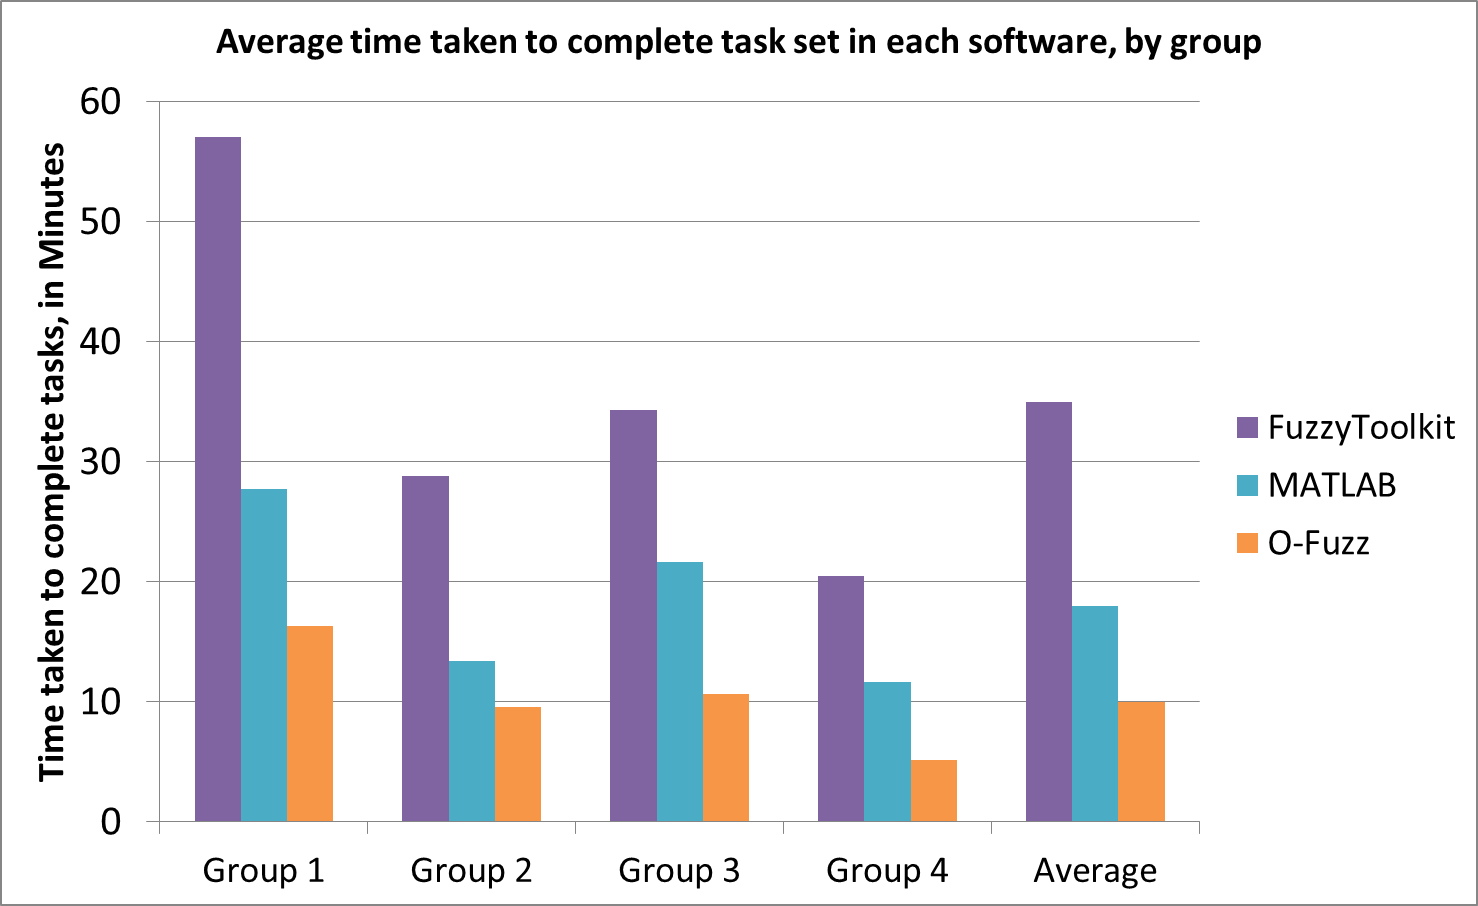
\includegraphics[width=0.8\textwidth]{images/timeTaken}
	\end{center}
	\vspace{-5mm}
	\captionsetup{justification=centering,margin=2cm}
	\caption{Bar chart of average time taken to complete the task set in the different software systems, by group}
	\label{fig:times}
	\vspace{-10mm}
\end{figure}
\newpage 
\noindent 						
Whilst the time taken to complete the tasks was a strong indicator of the success of the software system, it was also important to ask the participants which system they \emph{enjoyed} using the most. The results for this were conclusive, with 95.7\% of participants (across all categories) claiming FuzzyToolkitUoN was the piece of software they enjoyed using the least. The main reasons for this were the command line interface being difficult to use, visualisations of the system difficult to access, the necessity to constantly refer to the large documentation manual, and that it was conceptually confusing for many computer novices. 

\begin{figure}[ht!]
	\begin{center}
		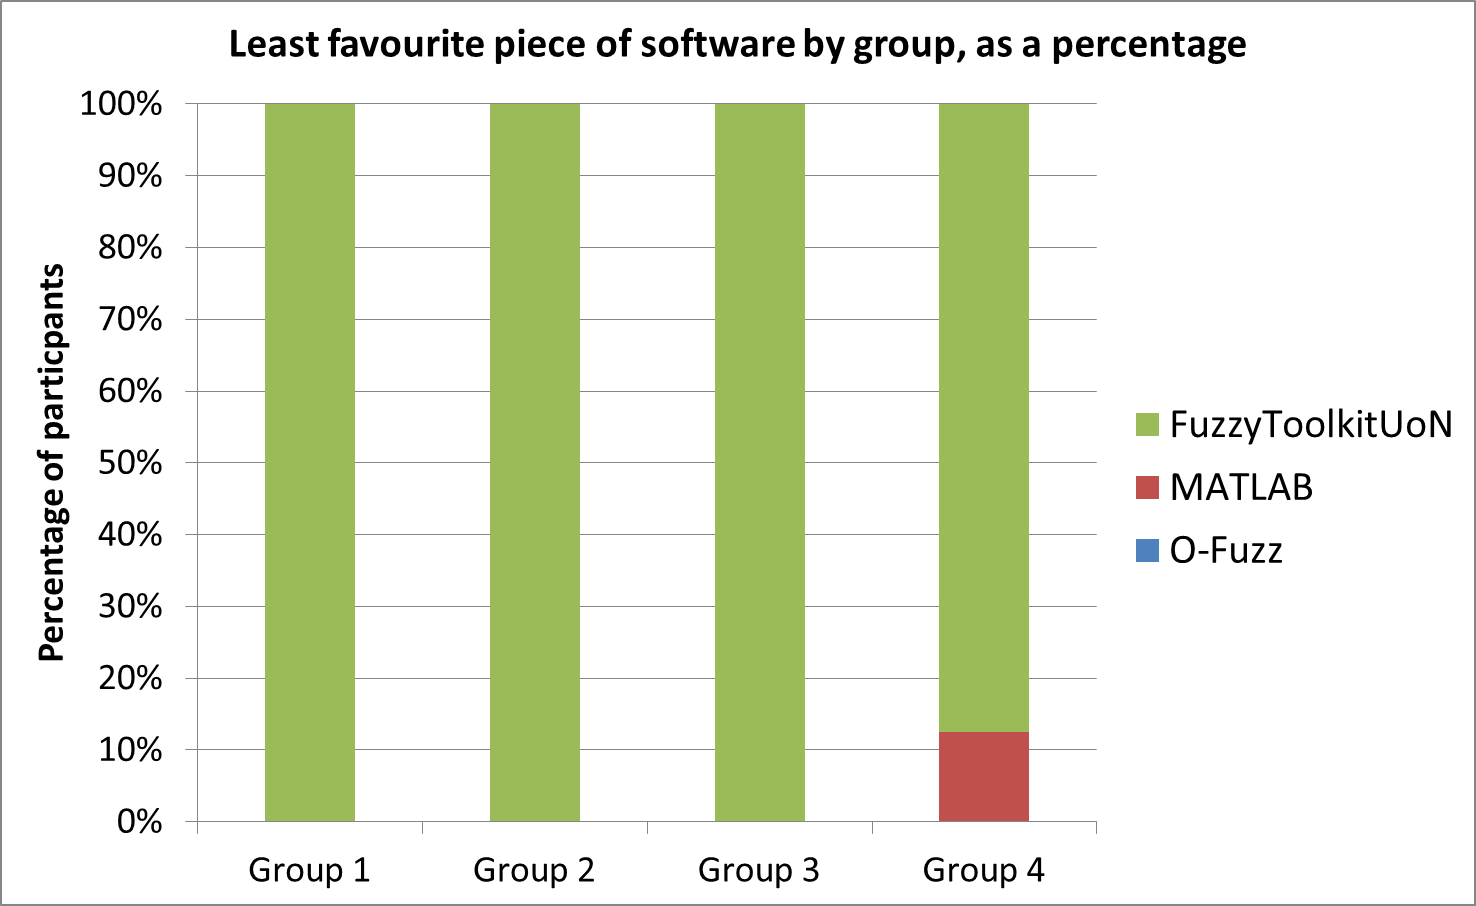
\includegraphics[width=0.8\textwidth]{images/leastFav}
	\end{center}
	\vspace{-5mm}
	\captionsetup{justification=centering,margin=2cm}	
	\caption{The percentage of users claiming each piece of software to by their least favourite}
	\label{fig:leastFavour}
	\vspace{-2mm}
\end{figure}
\noindent 
The piece of software that was most favoured by the test participants, was the system proposed in this report, o-Fuzz. Of the total participants, 65\% claimed o-Fuzz to be their favourite software, with 30\% saying it was MATLAB, and 4\% saying FuzzyToolkitUoN (a single person). A decomposition of favourite software, across the separate groups, can be seen in figure \ref{fig:mostLiked}
			
\begin{figure}[ht!]
	\begin{center}
		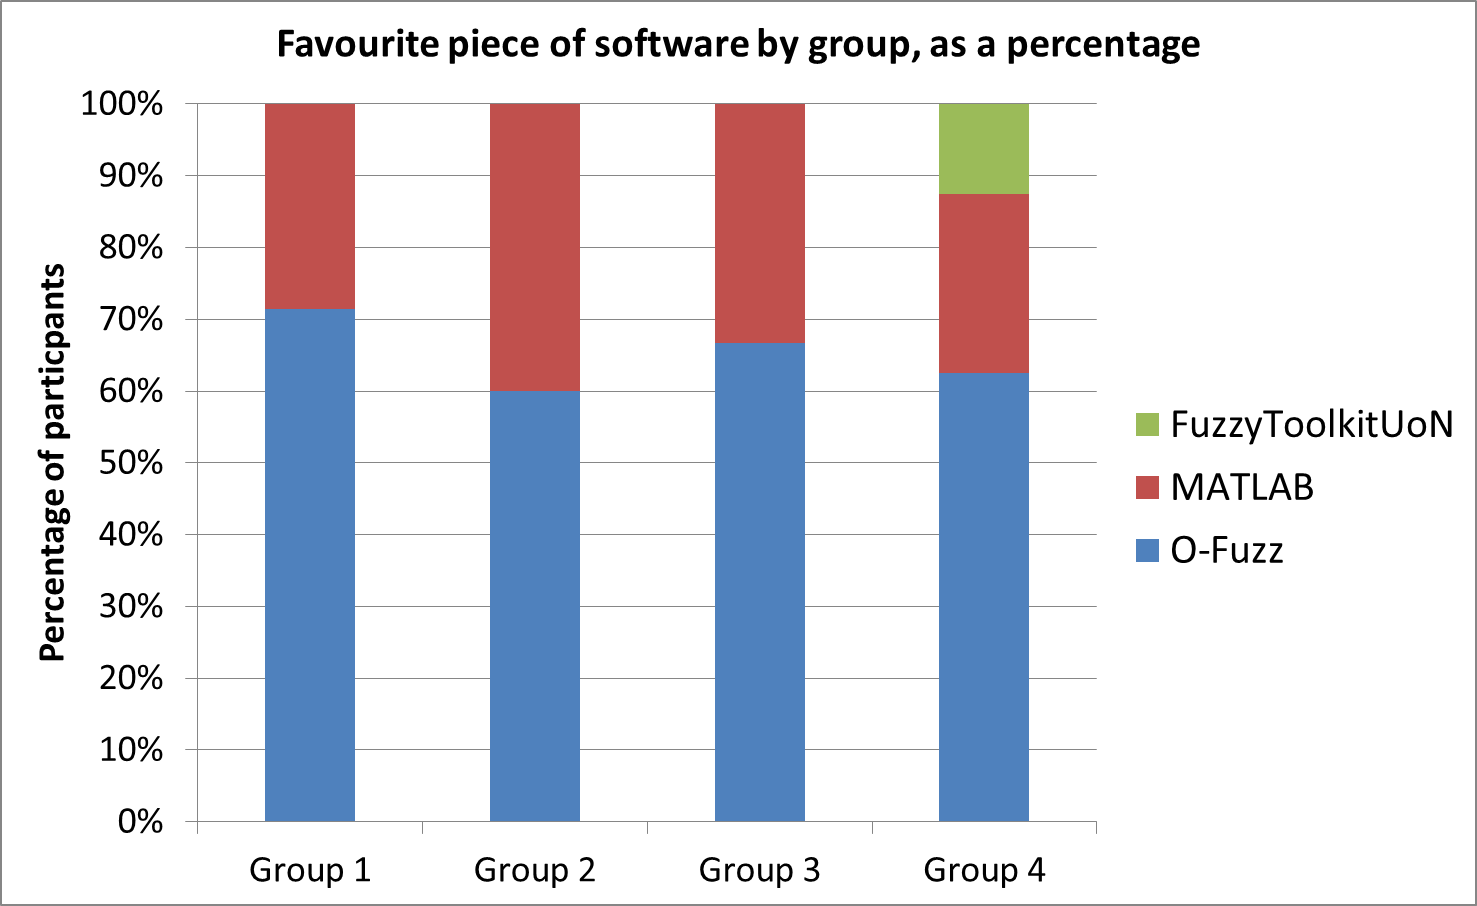
\includegraphics[width=0.8\textwidth]{images/mostFav.png}
	\end{center}
	\vspace{-5mm}
	\captionsetup{justification=centering,margin=2cm}	
	\caption{The percentage of users claiming each piece of software to by their most favourite}
	\label{fig:mostLiked}
	\vspace{-2mm}
\end{figure}
\noindent 
When questioned as to the preference of this new system, most users agreed that the interface was both extremely simple to navigate, and visually appealing. It was also mentioned that there was a natural flow to the software. By this, they meant that each task in the software lead onto the next very intuitively. For instance, the adding of a variable would be one distinct task, but the adding of membership functions would be a separate task nested inside this task. This meant that the conceptually distinct parts of the system were separate, but the system had a ``waterfall'' style flow to it. Many of the novice users also commended the system on it's help system, specifically mentioning how this was much more intuitive than checking the huge documentation manual provided with FuzzyToolkitUoN.\ \\
\ \\
It is worth noting that the single result for FuzzyToolkitUoN as favourite software came from a user that was extremely proficient in R, and specifically FuzzyToolkitUoN, and knew many commands from memory. This was also the same person that rated MATLAB as their least favourite piece of software, claiming that it was far too cluttered and aesthetically unappealing.
	

\subsection{Successes and Limitations of the Project}
% Successes:
% Fulfills its main two goals
% Easy to pick up by a novice user 
% Easily expandable
% Deals with errors well
% responsiveness

% Limitations
% Backend did not provide a lot of functionality -> Get new backend/API Layer
% probably a bug somewhere -> unit testing next time
% doesn't work on mobiles -> no action